\documentclass{scrartcl}

\usepackage[utf8]{inputenc}
\usepackage{color}
\usepackage{xcolor}

\usepackage{graphics}           % Add pictures to the document
\usepackage{graphicx}           % Add pictures to the document
\usepackage{subfigure}          % 2 pictures side by side

\title{Dokumentation ProductAR}
\author{Maximilian Rehberger}
\date{\today}

\setcounter{secnumdepth}{4}
\setcounter{tocdepth}{4}

\definecolor{darkcerulean}{rgb}{0.03, 0.27, 0.49}
\definecolor{frenchblue}{rgb}{0.0, 0.45, 0.73}
\definecolor{babyblueeyes}{rgb}{0.63, 0.79, 0.95}

\addtokomafont{section}{\color{darkcerulean}}
\addtokomafont{subsection}{\color{frenchblue}}
\addtokomafont{subsubsection}{\color{babyblueeyes}}

\graphicspath{ {./img/} }                % Path to images

\begin{document}


\maketitle

\newpage


\renewcommand*\contentsname{}
\section{Inhaltsverzeichnis}
\tableofcontents{}


\newpage

\section{Einleitung}

\subsection{Zweck}

Produkte können zum Beispiel beim Einkaufen mit dem Smartphone gescannt werden und erkannt werden. Informationen werden angezeigt wie zum Beispiel Bilder oder ein Preisvergleich. Mithilfe der App soll man einen Barcode einscannen können und Informationen zu den Produkten erhalten. Weiterhin kann der Nutzer ein Produkt in Augmented Reality (AR) testen und sieht somit wie es in Wirklichkeit aussehen wird, wenn er es kaufen würden.

\newpage

\section{Allgemeine Übersicht}

\subsection{Beschreibung Ausgangssituation}

Es gibt bereits viele Shopping-Apps wie zum Beispiel Ikea, H\&M oder S'Oliver. Das Problem ist, dass jeder am Ende für jedes Geschäft eine eigene App auf dem Smartphone hat. Diese App soll die Möglichkeiten geben mehrere unterschiedliche Produkte in einer App zu speichern und zu verwalten. Also eine App für alle Produkte.

\subsection{Produkteinsatz}

 Die App kann zum Beispiel als Einkaufsliste oder Wunschliste für Produkte eingesetzt werden.
 Darüber hinaus bieten sich noch viele weitere Möglichkeiten.

\subsection{Produktumfeld}

Die App wird hauptsächlich im privaten Umfeld umgesetzt, beim Einkaufen in Geschäften oder Online-Einkauf.

\subsection{Produktfunktionalität}

Scannen von Produkten, Informationen zu Produkten, Preisvergleich, Bilder hochladen für Produkte, Produkte in AR testen.

\subsection{Personas}

\subsubsection{Nutzer}

\subsubsection{Verkäufer}

\subsubsection{Admin}


\newpage

\section{Architekturkonzept und Entwurf}

\subsection{Ursprüngliches Architekturkonzept}

\begin{figure}[h]
\centering
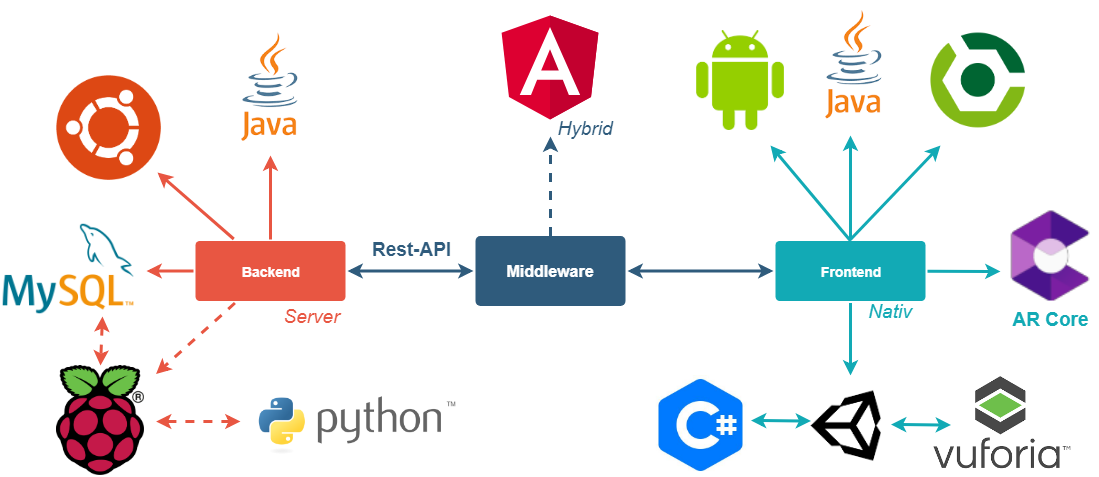
\includegraphics[width=380px]{img/Architekturkonzept.png}
\caption{Ursprüngliches Architekturkonzept}
\end{figure}

\subsection{Aktualisiertes Architekturkonzept}

\begin{figure}[h]
\centering
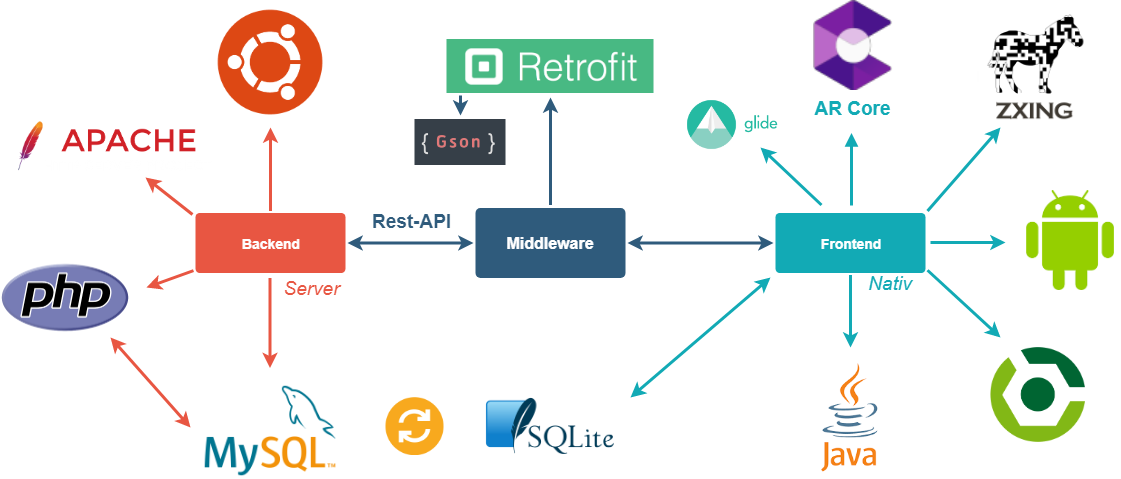
\includegraphics[width=380px]{img/ArchitekturkonzeptNew.png}
\caption{Aktualisiertes Architekturkonzept}
\end{figure}

\newpage

\subsection{Anfängliche Skizze Datenbankentwurf}

\subsubsection{MySQL Datenkbank (Remote)}

Ursprünglich war geplant, dass die Daten ausschließlich auf dem Server in einer MySQL Datenbank gespeichert werden.

\begin{figure}[h]
\centering
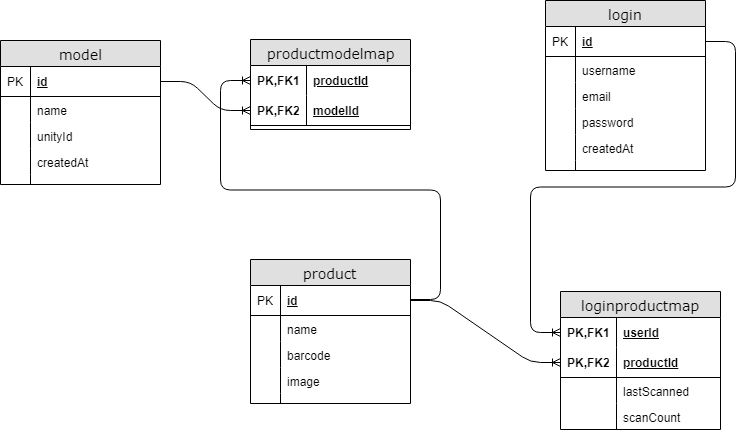
\includegraphics[width=380px]{img/Skizze_Datenbank_1.png}
\caption{Anfängliche Skizze Datenbankentwurf}
\end{figure}

\newpage

\subsection{Anfängliche Skizze Java Klassen}

\begin{figure}[h]
\centering
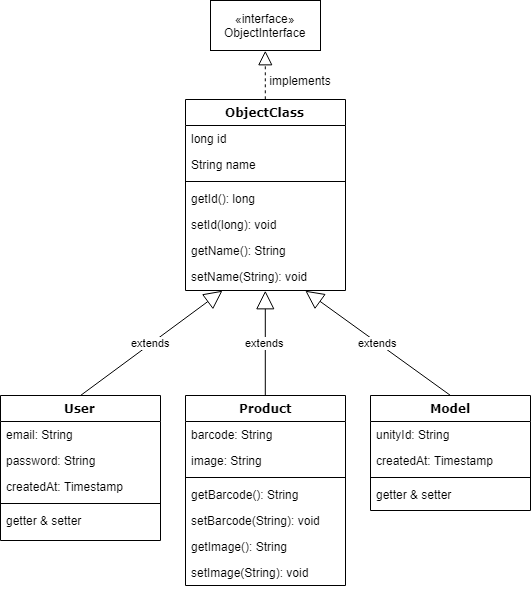
\includegraphics[width=320px]{img/Skizze_Java_1.png}
\caption{Anfängliche Skizze Datenbankentwurf}
\end{figure}

\newpage

\subsection{Endgültige Skizze Datenbankentwurf}

\subsubsection{SQLite Datenbank (Lokal)}

\begin{figure}[h]
\centering
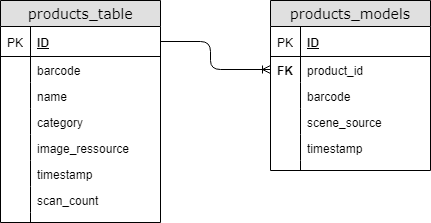
\includegraphics[width=180px]{img/Skizze_Datenbank_SQLite.png}
\caption{Skizze Datenbankentwurf: SQLite}
\end{figure}

\subsubsection{MySQL Datenbank (Remote)}

\begin{figure}[h]
\centering
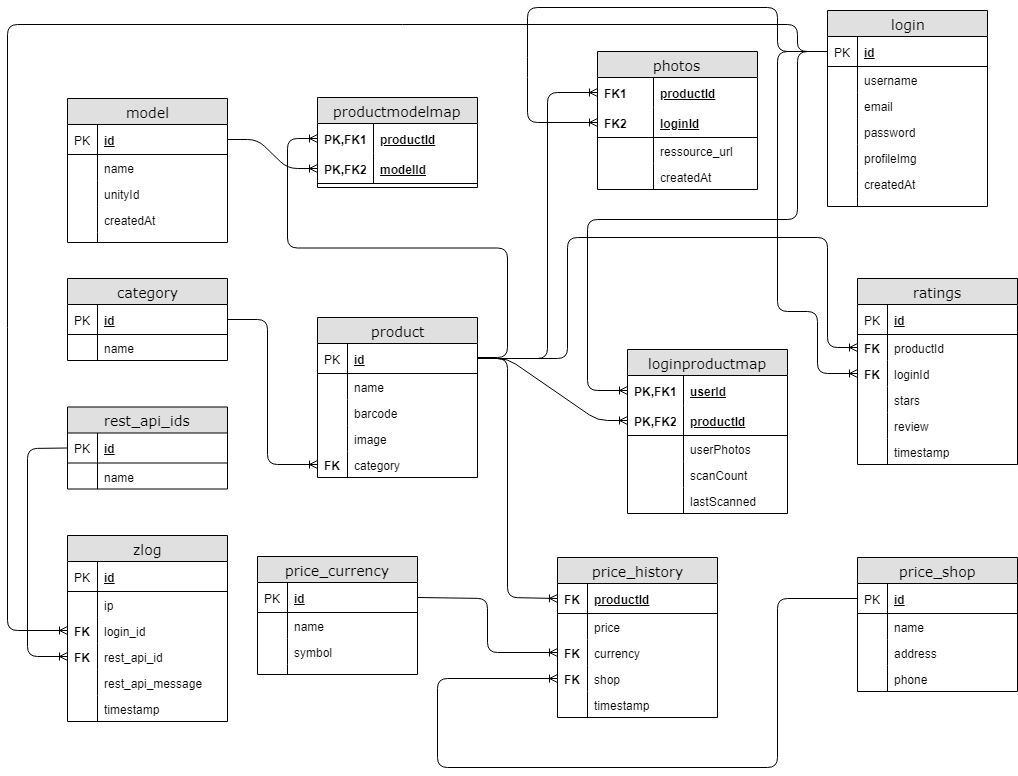
\includegraphics[width=380px]{img/Skizze_Datenbank_2.png}
\caption{Aktualisierte Skizze Datenbankentwurf: MySQL}
\end{figure}

\newpage

\subsection{Endgültige Skizze Java Klassen}

\begin{figure}[h]
\centering
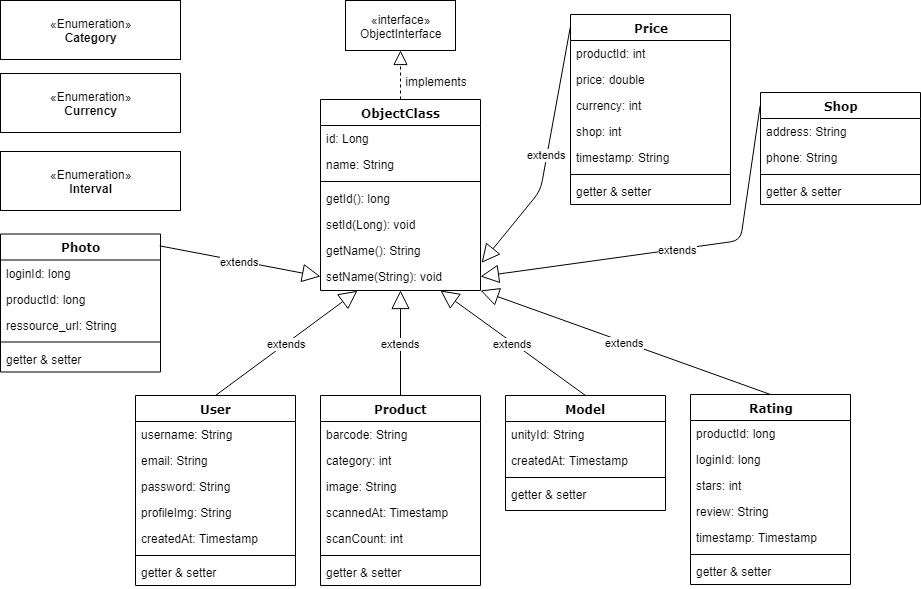
\includegraphics[width=380px]{img/Skizze_Java_New.png}
\caption{Aktualisierte Skizze: Java Klassen}
\end{figure}

\subsection{Übersicht Backend Server}

\subsection{Übersicht REST API}

\subsection{Technische Entscheidungen}

\subsubsection{Warum Android?}

\subsubsection{Welche Androidversion?}

\subsubsection{Welche Entwicklungsumgebung?}

Android Studio.

\subsubsection{Warum eine MySQL Datenbank?}

\subsubsection{Warum eine REST API?}

\subsubsection{Vergleich mit Alternativlösungen}

\paragraph{Firebase von Google}

\paragraph{Alternative Datenbankmodelle}


\newpage

\section{Technische Dokumentation}

\subsection{Android Manifest}

\subsection{Java Interfaces}

\subsubsection{ObjectInterface}

\subsubsection{ScanResultReceiver}

\subsubsection{IRetrofitCRUD}

\subsubsection{JsonPlaceHolderApi}

\subsection{Java Klassen}

\subsubsection{Objekt Klassen}

\paragraph{Object Class (Abstract)}

\paragraph{Product}

\paragraph{User}

\paragraph{Model}

\paragraph{Photo}

\paragraph{Price}

\paragraph{Shop}

\paragraph{Category (Enum)}

\paragraph{Currency (Enum)}

\paragraph{Interval (Enum)}

\subsubsection{Aktivity Klassen}

\paragraph{MainActivity}

\paragraph{SplashScreen}

\paragraph{ProductArActivity}

\paragraph{ProductScanActivity}

\paragraph{CaptureActivityPortrait}

\paragraph{LastScannedProductsActivity}

\paragraph{CreateProductActivity}

\paragraph{ProductDetailActivity}

\paragraph{ProductPhotoGalleryActivity}

\paragraph{ProductPhotoDetailActivity}

\paragraph{CreatePriceActivity}

\paragraph{PriceHistoryActivity}

\paragraph{RegisterActivity}

\paragraph{LoginActivity}

\paragraph{ProfileActivity}

\paragraph{SettingsActivity}

\paragraph{InfoActivity}

\subsubsection{Adapter Klassen}

\paragraph{ProductListAdapter}

\paragraph{PhotoAdapter}

\subsubsection{Hilfs Klassen}

\paragraph{GeneralHelper}

\paragraph{BarcodeHelper}

\paragraph{QRCodeHelper}

\paragraph{LoginHelper}

\paragraph{SettingsHelper}

\paragraph{ImageHelper}

\paragraph{PhotoHelper}

\paragraph{UploadHelper}

\paragraph{PriceHelper}

\subsubsection{Fragment Klassen}

\paragraph{ScanFragment}

\paragraph{CustomArFragment}

\subsubsection{Retrofit Schnittstelle}

\subsubsection{Network Monitor}

\subsubsection{Background Service}

\subsubsection{Notifications}

\subsection{Ressourcen}

\subsubsection{Layout}

\subsubsection{Drawable Icons}

\subsubsection{App Icon}

\subsubsection{Animation}

\subsubsection{Menu}

\subsubsection{Assets}

\subsubsection{Values}

\subsection{Rest Api}


\newpage

\section{Veröffentlichung im Google Play Store}

\subsection{Store Eintrag}

\subsection{Alpha Test}

\subsection{Beta Test}


\newpage

\section{Zukünftige Entwicklungen}


\newpage

\section{Fazit}


\newpage

\section{Verwendete Technologie, Frameworks und Software}


\newpage

\section{Verlinkung Repositories}


\newpage

\section{Verlinkung Tutorials}


\newpage

\section{Quellenangabe}


\end{document}
